\chapter{Network}
\section{Proprietà dei grafi}
Quando le dimensioni dei grafi iniziano a crescere risulta difficile
rappresentarli in modo chiaro e comprensibile. Per questo motivo, quando si
lavora con grafi di grandi dimensioni, essi vengono rappresentati tramite
delle proprietà che ne descrivono la struttura, queste proprietà sono delle
statistiche descrittive che facilitano anche il confronto tra le reti.

Tra le proprietà più importanti troviamo:
\begin{itemize}
    \item \textbf{Lunghezza media dei cammini}: indica la lunghezza media dei
          cammini tra due nodi.
    \item \textbf{Diametro}: indica la lunghezza del cammino più lungo tra due
          nodi.
    \item \textbf{Grado di un nodo}: indica il numero di archi che partono o
          arrivano ad un nodo.
    \item \textbf{Coefficienti di clustering}: indicano la presenza di nodi
          vicini tra loro.
    \item \textbf{Centralità}: indica l'importanza di un nodo all'interno del
          grafo.
\end{itemize}
\subsection{Grado di un nodo}
\begin{definizione}[\textbf{Grado di un nodo}]
    Il \textbf{grado di un nodo} è il numero di archi che partono o arrivano ad
    un nodo. Nel caso di grafi diretti si parla di \textbf{grado uscente} o
    \textbf{out degree} e \textbf{grado entrante} o \textbf{in degree}.
\end{definizione}
Se si considera un grafo rappresentato attraverso una matrice di adiacenza, il
grado di un nodo può essere calcolato sommando i valori della riga o della
colonna corrispondente al nodo in questione. Nello specifico, se si considera
un grafo orientato, il grado uscente corrisponde alla somma dei valori della
riga corrispondente al nodo, mentre il grado entrante alla somma dei valori della
colonna ad esso associata.

Più in generale possiamo riassumere il calcolo del grado di un nodo come segue:
\begin{equation}
    \text{Outdegree}(i) = \sum_{j=1}^{n} A_{ij} \quad \text{e} \quad
    \text{Indegree}(i) = \sum_{j=1}^{n} A_{ji}
\end{equation}
dove $A_{ij}$ è l'elemento della matrice di adiacenza corrispondente al nodo
$i$ e $j$. Nel caso di grafi non orientati, il grado di un nodo corrisponde
alla somma dei valori della riga o della colonna corrispondente al nodo in
questione.

Il grado di un nodo rappresenta una misura locale del grafo, nel caso in cui
si voglia ottenere una misura globale del grafo si può calcolare il grado
medio dei nodi. Tale misura può essere calcolata come segue:
\begin{equation}
    \langle k \rangle = \frac{1}{n} \sum_{i=1}^{n} \text{Grado}(i)
\end{equation}
dove $n$ rappresenta il numero di nodi del grafo. Anche in questo caso, se il
grafo è orientato dobbiamo distinguere tra grado uscente e grado entrante.
\begin{nota}
    Possiamo calcolare il grado medio anche come segue:
    \begin{itemize}
        \item Nel caso di grafi non orientati:
              \begin{equation}
                  \langle k \rangle = \frac{2E}{n}
              \end{equation}
        \item Nel caso di grafi orientati:
              \begin{equation}
                  \langle k \rangle = \frac{E}{n}
              \end{equation}
    \end{itemize}
    dove $E$ rappresenta il numero di archi del grafo e $n$ rappresenta il
    numero di nodi.
\end{nota}
Una misura più rappresentativa della media dei gradi dei nodi è la \textbf{distribuzione
    dei gradi}. Possiamo definire $p(k)$ come la probabilità che un nodo abbia
grado $k$. Tale distribuzione può essere calcolata come segue:
\begin{equation}
    p(k) = \frac{n_k}{n}
\end{equation}
dove $n_k$ rappresenta il numero di nodi con grado $k$ e $n$ rappresenta il
numero totale di nodi del grafo. La distribuzione dei gradi può essere
rappresentata tramite un istogramma, in cui sull'asse delle ascisse vengono
inseriti i valori dei gradi, mentre sull'asse delle ordinate sono presenti i
valori di $p(k)$.
\begin{figure}[!ht]
    \centering
    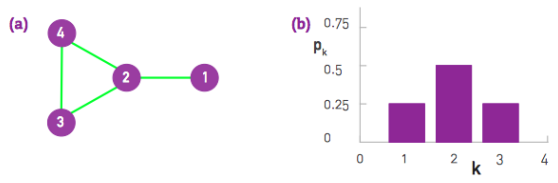
\includegraphics[width=0.7\textwidth]{./img/net/degreedist.png}
    \caption{Esempio di distribuzione dei gradi.}
    \label{fig:degree_distribution}
\end{figure}
\begin{nota}
    Questa distribuzione deve essere normalizzata, ovvero la somma di tutti i
    valori di $p(k)$ deve essere uguale a 1.
    \begin{equation*}
        \sum_{k=0}^{\infty} p(k) = 1
    \end{equation*}
\end{nota}
Il valore della distribuzione mi permette di rappresentare molti fenomeni: dalla
Il valore della distribuzione mi permette di rappresentare molti fenomeni: dalla
robustezza della rete, alle sue vulnerabilità.
\subsection{Cammino e distanza}
\begin{definizione}[\textbf{Cammino}]
    Un \textbf{cammino} è una sequenza di nodi in cui ciascun nodo è adiacente
    al successivo.
\end{definizione}
\begin{definizione}[\textbf{Distanza}]
    La \textbf{distanza} tra due nodi è definita come il numero minimo di archi
    che devono essere attraversati per andare da un nodo all'altro. Se i due
    nodi non sono collegati, la distanza è infinita.
\end{definizione}
Un modo semplice per calcolare la distanza tra due nodi è quello di utilizzare
l'algoritmo BFS (Breadth First Search).
\begin{definizione}[\textbf{Diametro}]
    Il \textbf{diametro} di un grafo è la distanza massima tra due nodi nel grafo.
\end{definizione}
\begin{definizione}[\textbf{Lunghezza media dei cammini}]
    La \textbf{lunghezza media dei cammini} è la media delle distanze tra tutti 
    i nodi del grafo. Tale misura può essere calcolata come segue nel caso di 
    un grafo orientato:
    \begin{equation}
        \langle d \rangle = \frac{1}{E_{max}} \sum_{i \neq j} d_{ij}
    \end{equation}
\end{definizione}
Mentre, nei grafi non orientati, la lunghezza media dei cammini può essere calcolata
come segue:
\begin{equation}
    \langle d \rangle = \frac{1}{2E_{max}} \sum_{i \neq j} d_{ij}
\end{equation}
dove $d_{ij}$ rappresenta la distanza tra i nodi $i$ e $j$ e $E_{max}$ rappresenta
il numero massimo di archi presenti nel grafo.
\subsection{Coefficienti di clustering}
\begin{definizione}[\textbf{Coefficienti di clustering}]
    I \textbf{coefficienti di clustering} sono una misura della presenza di nodi
    vicini tra loro. In particolare, il coefficiente di clustering di un nodo è una
    misura della probabilità che i vicini di un nodo siano collegati tra loro.
    Dato un nodo $i$ con grado $k_i$, il coefficiente di clustering locale è
    definito come segue (grafo non orientato):
    \begin{equation}
        C_i = \frac{2E_i}{k_i(k_i - 1)}
    \end{equation}
    dove $E_i$ rappresenta il numero di archi tra i $k_i$ vicini del nodo $i$.
    Se il grafo è orientato allora si divide per $2$ il coefficiente.
\end{definizione}

Il valore di questo coefficiente può variare tra 0 e 1. Nel caso in cui il
coefficiente sia uguale a 1, significa che tutti i vicini del nodo $i$ sono
collegati tra loro. Nel caso in cui il coefficiente sia uguale a 0, significa
che nessun vicino del nodo $i$ è collegato ad un altro vicino.

Questa misura rappresenta la densità locale di un grafo. Per ottenere una
misura \textbf{globale} della densità del grafo, possiamo calcolare il
\textbf{coefficiente di clustering medio}. Tale misura può essere calcolata come
segue:
\begin{equation}
    \langle C \rangle = \frac{1}{n} \sum_{i=1}^{n} C_i
\end{equation}
dove $\langle C \rangle$ si può interpretare come la probabilità che due vicini
di un nodo, selezionato in modo casuale, siano collegati tra loro.
\begin{definizione}[\textbf{Hub}]
    Un \textbf{hub} è un nodo che ha un grado molto alto, ovvero è connesso a
    molti altri nodi e ha una probabilità molto bassa di occorrere nella rete.
\end{definizione}
\begin{esempio}
    Vediamo ora un esempio di come commentare lo studio di un grafo dal punto di
    vista delle statistiche descrittive. Supponiamo di avere ottenuto un
    i seguenti grafici:
    \begin{figure}[!ht]
        \centering
        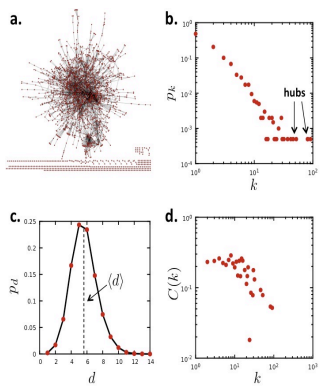
\includegraphics[width=0.5\textwidth]{./img/net/esempio1.png}
        \caption{Esempio di grafici ottenuti dallo studio di un grafo.}
        \label{fig:graphstats}
    \end{figure}

    La distribuzione di grado, riportata nel grafico $b$ della figura \ref{fig:graphstats},
    ci permette di ottenere informazioni in più rispetto alla media. Questo
    perché la media è uno stimatore distorto, sarebbe meglio utilizzare la
    mediana. Inoltre la distribuzione di grado permette di studiare gli \textbf{hub}.

    Il grafico $c$ della figura \ref{fig:graphstats} ci permette di ottenere
    informazioni sul diametro del grafo, sulla lunghezza media dei cammini.

    Il coefficiente di clustering medio permette di capire quanto sono connessi
    i vicini di un nodo estratto casualmente. Il grafico del coefficiente di
    clustering, riportato in figura \ref{fig:graphstats} $d$ mostra le relazioni
    tra grado e clustering. In questo esempio, i nodi spoke hanno un coefficiente
    di clustering maggiore quindi il vicinato è molto connesso, sintomo
    organizzazione gerarchica.

    Con questi ragionamenti si riesce ad effettuare inferenze sul comportamento
    che si ottiene se si dovesse rimuovere un nodo.
\end{esempio}
\section{Centralità del grafo}
La centralità di un nodo è una misura dell'importanza di un nodo all'interno
del grafo. Questa misura può essere calcolata in diversi modi, in base a
diversi criteri. Tra le misure di centralità più comuni troviamo:
\begin{itemize}
    \item \textbf{Degree}
    \item \textbf{Betweeness}
    \item \textbf{Closeness}
    \item \textbf{Autovettori}
    \item \textbf{Pagerank}
\end{itemize}
\subsection{Degree}
Una delle prime possibilità di misurare la centralità di un nodo è quella di
utilizzare il grado del nodo. Questa misura è particolarmente utile nel caso di
reti sociali, in cui il grado di un nodo corrisponde al numero di amici che
il nodo ha.
\begin{equation}
    C_D(i) = \sum_{j=1}^{n} x_{ij}
\end{equation}

Nel caso di grafo orientato, possiamo distinguere tra grado entrante e grado
uscente.

\begin{equation}
    C_{D_{in}}(i) = \sum_{j=1}^{n} x_{ji} \quad \text{e} \quad
    C_{D_{out}}(i) = \sum_{j=1}^{n} x_{ij}
\end{equation}
La centralità massima per un nodo è $n - 1$.

Questa misura può essere normalizzata
dividendo la centralità di grado per il numero di nodi meno uno.
\begin{equation*}
    {C_D}_{norm} (i)= \frac{C_D(i)}{n-1}
\end{equation*}

Oltre alla misura di centralità di grado, possiamo calcolare la \textbf{centralizzazione}.
\begin{definizione}[\textbf{Centralizzazione}]
    La \textbf{centralizzazione} di un grafo è una misura di quanto è centrale il
    nodo con massima centralità rispetto alla centralità di tutti gli altri.
    In particolare, la centralizzazione
    di un grafo è massima quando il nodo con centralità massima ha una centralità
    molto più alta rispetto agli altri nodi del grafo.
\end{definizione}

La centralizzazione di un grafo può essere calcolata come usando la formula di Freeman:
\begin{equation}
    C_D = \frac{\sum_{i=1}^{n} C_D(n^\ast) - C_D(i)}{(n - 1)(n - 2)}
\end{equation}
dove:
\begin{itemize}
    \item $C_D(n^\ast)$: corrisponde alla centralità massima di un nodo del grafo.
    \item $C_D(i)$: corrisponde alla centralità del nodo $i$.
    \item $n$: corrisponde al numero di nodi del grafo.
\end{itemize}
\subsection{Betweeness}
Un altra misura di centralità è la \textbf{betweeness}, ovvero il nodi più
rilevanti sono quelli che fanno da ponte tra due gruppi di nodi. Posso anche
vederli come nodi che fanno da collo di bottiglia. La betweeness di un nodo
può essere calcolata come segue:
\begin{equation}
    C_B(i) = \sum_{i \neq j \neq k} \frac{g_{jk}(i)}{g_{jk}}
\end{equation}
dove:
\begin{itemize}
    \item $g_{jk}(i)$: corrisponde al numero di \textit{path} tra i
          nodi $j$ e $k$ nella rete tale che il cammino passa per il nodo $i$.
    \item $g_{jk}$: corrisponde al numero di \textit{path} tra i nodi
          $j$ e $k$.
\end{itemize}
In questo caso, la centralità è massima se un nodo ha alta capacità di unire
gruppi. Mentre la centralità tende a $0$ il nodo non collega nessuno.

Viene successivamente fatta una seconda normalizzazione, questa volta sui nodi,
per rendere indipendentemente dalla dimensione del grafo. Questo può essere
espresso nel caso di un grafo non orientato come segue:
\begin{equation}
    {C_B}_{norm}(i) = \frac{C_B(i)}{(n - 1)(n - 2)}
    {C_B}_{norm}(i) = \frac{C_B(i)}{(n - 1)(n - 2)}
\end{equation}
mentre nel caso di un grafo orientato come segue:
\begin{equation}
    {C_B}_{norm}(i) = \frac{C_B(i)}{\frac{(n - 1)(n - 2)}{2}}
    {C_B}_{norm}(i) = \frac{C_B(i)}{\frac{(n - 1)(n - 2)}{2}}
\end{equation}
\subsection{Closeness}
La centralità misurata come \textbf{closeness} è una misura della vicinanza di
un nodo agli altri nodi del grafo. Questa misura può essere calcolata come segue:
\begin{equation}
    C_C(i) = \frac{1}{\sum_{j=1}^{n} d_{ij}}
\end{equation}
Corrisponde alla misura di un vertice in merito alla sua efficienza nel
comunicare l'informazione, mentre la betweeness è una misura l'efficacia di un
nodo nel trasmettere un'informazione.
nodo nel trasmettere un'informazione.

Questa misura può essere normalizzata come segue:
\begin{equation}
    {C_C}_{norm}(i) = \frac{C_C(i)}{n - 1}
    {C_C}_{norm}(i) = \frac{C_C(i)}{n - 1}
\end{equation}
\subsection{Autovettori}
La misura di centralità calcolata utilizzando il grado del nodo rappresenta una
misura locale del grafo. Inoltre, questa misura non tiene conto del ruolo dei
nodi con cui il nodo è collegato. Per ottenere una misura globale della
centralità del nodo, possiamo utilizzare la \textbf{centralità di autovettori}.

La centralità di autovettori è una misura della centralità di un nodo in base
al ruolo dei nodi con cui è collegato, ovvero un nodo è importante se è
collegato ad altri nodi importanti.

Questa misura può essere calcolata come segue:
\begin{equation}
    C_A(i) = \frac{1}{\lambda} \sum_{j=1}^{n} A_{ij} C_A(j)
\end{equation}
dove $A$ è la matrice di adiacenza del grafo e $\lambda$ è l'autovalore
corrispondente all'autovettore dominante della matrice di adiacenza. 

A differenza della misura basata sul grado, un nodo che ha un alto grado ma è
collegato a nodi poco importanti avrà una centralità di autovettori bassa. Al
contrario, un nodo che ha un grado basso ma è collegato a nodi molto importanti
avrà una centralità di autovettori alta.
\subsection{Pagerank}
La centralità basata su \textbf{pagerank} è una specializzazione della centralità
di autovettori. Nello specifico questa misura è stata sviluppata per misurare
la centralità di un grafo orientato.

L'assunzione su cui si basa questa misura è che un arco tra il nodo $i$ e il
nodo $j$ rappresenta un voto del nodo $i$ al nodo $j$. Se i due nodi sono connessi
attraverso un arco, la probabilità che i due nodi siano in qualche modo collegati
è maggiore.

L'idea alla base di questa misura è che un nodo $i$ è influenzato dall'importanza
dai nodi che si collegano a lui, in altre parole, gli altri nodi votano per il
nodo $i$.

Il coefficiente di PageRank associato a un nodo $i$ può essere calcolato come:
\begin{equation}
    P(i) = \sum_{(j, i) \in E} \frac{P(j)}{O_j}
\end{equation}
dove $O_j$ rappresenta il numero di archi uscenti dal nodo $j$ e $P$ rappresenta
il vettore di PageRank.

Il vettore di PageRank può essere calcolato andando a risolvere un sistema
lineare di $n$ equazioni in $n$ variabili. In particolare, possiamo scrivere il
vettore di PageRank $P = (P(1), \dots, P(n))^T$ come segue:
\begin{equation}
    P = A^T \cdot P
\end{equation}
dove $A$ è la matrice di adiacenza del grafo definita come:
\begin{equation*}
    A_{ij} = \begin{cases}
        \frac{1}{O_i} & \text{se esiste un arco da $i$ a $j$} \\
        0             & \text{altrimenti}
    \end{cases}
\end{equation*}
A questo punto, la soluzione del problema può essere ottenuta utilizzando un
algoritmo iterativo che restituisce gli autovettori della matrice di adiacenza
normalizzata.

Il problema è che per garantire la convergenza di questo algoritmo è necessario
rispettare due condizioni:
\begin{itemize}
    \item Si ha un unico autovalore massimo che deve essere $1$.
    \item $P$ è l'autovettore di modulo massimo di $A$.
    \item Si ha un unico autovalore massimo che deve essere $1$.
    \item $P$ è l'autovettore di modulo massimo di $A$.
\end{itemize}

Un'altro possibile metodo per risolvere questo problema è quello di utilizzare
la \textbf{Markov Chain}. In questo caso ogni nodo rappresenta uno stato della
catena e ogni arco rappresenta una transizione che permette di passare da uno
stato all'altro con una certa probabilità.

Questa soluzione permette di simulare la navigazione dell'utente nel web
attraverso diverse pagine e di calcolare la probabilità che l'utente raggiunga
un nodo partendo da un altro nodo.

Per questa soluzione viene utilizzata la matrice di transizione di probabilità
$A$ definita in precedenza, dove ogni elemento $A_{ij}$ rappresenta la probabilità
che l'utente passi dal nodo $i$ al nodo $j$.

A questo punto, partendo da una probabilità iniziale $P_0 = (P_0(1), \dots, P_0(n))^T$
e la matrice di transizione $A$ abbiamo:
\begin{equation*}
    \sum_{i = 1}^n P_0(i) = 1
\end{equation*}
Inoltre, se la matrice $A$ soddisfa la seguente proprietà:
\begin{equation*}
    \sum_{j = 1}^n A_{ij} = 1
\end{equation*}
allora la matrice $A$ è stocastica.

Dal teorema della Markov Chain sappiamo che se la catena di Markov è definita da
una matrice di transizione stocastica allora è caratterizzata da un unica
distribuzione di probabilità stazionaria se $A$ è irriducibile e aperiodica.
\begin{nota}
    Una distribuzione di probabilità stazionaria garantisce che dopo un certo
    numero di passi la probabilità di raggiungere un nodo da tutti gli altri
    nodi non cambia.
\end{nota}
Per garantire questo devono essere verificate le seguenti condizioni:
\begin{itemize}
    \item La matrice $A$ deve essere \textbf{stocastica}, ovvero la somma di
          ogni riga deve essere uguale a 1.
          \begin{equation*}
              \sum_{j = 1}^n A_{ij} = 1
          \end{equation*}
          Un problema in questo caso è rappresentato da una pagina che non ha
          link uscenti, essa sarebbe rappresentata da una riga di $0$. Si hanno
          due possibili soluzioni:
          \begin{itemize}
              \item Aggiungere un arco uscente per ogni nodo che non rispetta la
                    condizione.
              \item Rimuovere tutte le pagine che non hanno link uscenti.
          \end{itemize}
    \item \textbf{Irriducibilità}: se il grafo è fortemente connesso.
    \item \textbf{Aperiodicità}: se tutti gli stati della catena sono aperiodici,
          ovvero se non fa parte di cicli.
\end{itemize}
Una soluzione alle problematiche relative alla irriducibilità e aperiodicità
si ottiene aggiungendo un arco da ogni nodo a tutti gli altri nodi del grafo con
una probabilità di transizione molto bassa controllata da un parametro $d$:
\begin{equation}
    P_{i} = (1 - d) + d \cdot \sum_{(j, i) \in E}\frac{P(j)}{O_j}
\end{equation}

Il coefficiente di PageRank $P_i$ può essere calcolato risolvendo il seguente
sistema di equazioni:
\begin{equation}
    \left[
        \begin{array}{c}
            P_1    \\
            \vdots \\
            P_n
        \end{array}
        \right] = d \cdot \left[
        \begin{array}{ccc}
            A_{11} & \dots  & A_{1, n} \\
            \vdots & \ddots & \vdots   \\
            A_{n1} & \dots  & A_{nn}
        \end{array}
        \right] + (1 - d) \cdot \left[
        \begin{array}{c}
            1      \\
            \vdots \\
            1
        \end{array} \right]
\end{equation}
Sotto la seguente condizione:
\begin{equation*}
    \sum_{i}^n P_i = 1
\end{equation*}
\subsubsection{Altri metodi per calcolare la centralità}
Oltre alle metriche appena presentate, esistono altri metodi per calcolare la
centralità. Tra questi metodi troviamo:
\begin{itemize}
    \item \textbf{Reciprocity}: ovvero il rapporto tra il numero di relazioni che
          sono reciproche (l'arco è in entrambe le direzioni) e il numero totale
          di relazioni. Con relazione si intende il fatto che due nodi siano
          collegati indipendentemente dalla direzione dell'arco. Chiaramente ha
          senso solo nelle reti orientate.
    \item \textbf{Density}: ovvero il rapporto tra il numero di archi presenti nel
          grafo e il numero massimo di archi che potrebbero essere presenti.
          Il numero massimo di archi che potrebbero essere presenti è dato da
          $\frac{n(n-1)}{2}$ nel caso di grafi non orientati e $n(n-1)$ nel caso
          di grafi orientati.
\end{itemize}
\section{Community detection}
\begin{definizione}[\textbf{Community}]
    Le \textbf{community} sono dei sottogruppi di oggetti che condividono delle
    proprietà.
\end{definizione}
Ci interessa l'identificazione delle community per:
\begin{itemize}
    \item Scoprire funzionalità relative agli oggetti.
    \item Studiare interazioni tra gruppi.
    \item Inferire sui collegamenti che ci sono tra community ex: social Network.
    \item Inferire dei dati mancanti di un nodo dalla sua community.
\end{itemize}
\begin{esempio}
    Un esempio di community sono quelle presenti nei social network. In questo caso,
    le community sono degli insiemi di utenti che effettuano delle interazioni
    tra di loro, come ad esempio relazioni di amicizia, oppure mettere like a
    uno stesso post.
\end{esempio}
Non esiste una definizione unica di community, ma esistono diversi criteri per
identificarle. Ad esempio, se consideriamo la figura \ref{fig:community}, possiamo
riconoscere in modo diverso le community in base al criterio che utilizziamo.
In questo caso, possiamo identificare:
\begin{itemize}
    \item 3 community quelle rappresentate dalle componenti connesse.
    \item 9 community se le consideriamo come insiemi di nodi vicini tra loro,
          insiemi densi di nodi.
\end{itemize}
\begin{figure}[!ht]
    \centering
    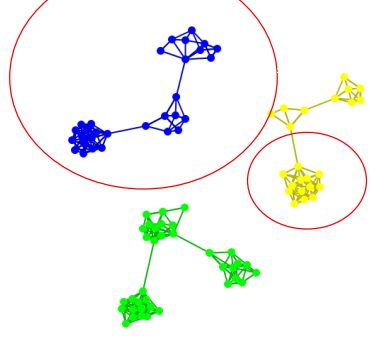
\includegraphics[width=0.3\textwidth]{./img/net/community.png}
    \caption{Esempio di community.}
    \label{fig:community}
\end{figure}

Una volta identificate le community, possiamo studiare le relazioni tra di loro.
Una prima osservazione può essere fatta sul fatto che le community possono
essere:
\begin{itemize}
    \item \textbf{Disgiunte}: non condividono nessun nodo.
    \item \textbf{Sovrapposte}: condividono alcuni nodi, anche detto \textbf{overlap}.
\end{itemize}
\begin{figure}[!ht]
    \centering
    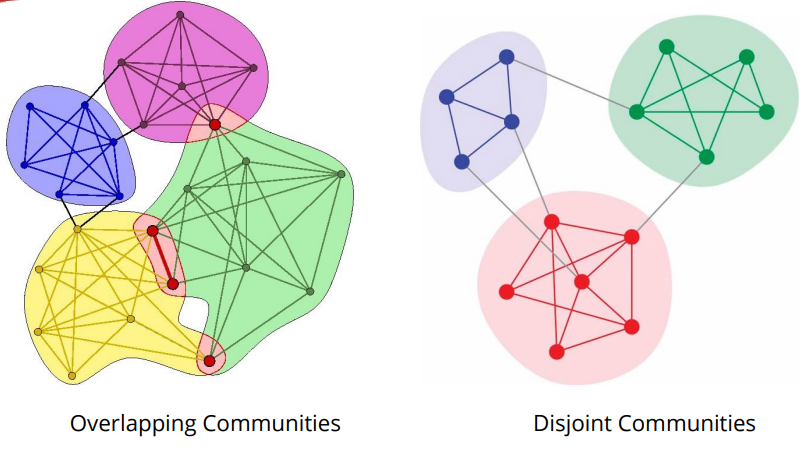
\includegraphics[width=0.3\textwidth]{./img/net/overlap.png}
    \caption{Esempio di community che si sovrappongono.}
    \label{fig:overlap}
\end{figure}
\subsection{Criteri per identificare le community}
Esistono diversi criteri per identificare le community, ognuno dei quali si adatta
a diversi tipi di studi che si vogliono effettuare. Questi criteri possono essere
suddivisi nelle seguenti categorie  ordinate dalla più stringente alla meno
stringente:
\begin{itemize}
    \item \textbf{Node-centric}: si creano delle community sulla base delle
          caratteristiche sui singoli nodi.
    \item \textbf{Group-centric}: si creano delle community dal punto di vista
          di un gruppo. Il gruppo deve rispettare un determinato criterio senza
          considerare i singoli nodi.
    \item \textbf{Network-centric}: si valuta il criterio nell'interezza della rete.
    \item \textbf{Hierarchy-centric}: si costruisce una struttura gerarchica delle
          community basata sulla topologia della rete.
\end{itemize}
\subsubsection{Node-centric}
Questo criterio si basa sulla ricerca di caratteristiche comuni tra i singoli
nodi. In particolare, i nodi che fanno parte della stessa community devono
rispettare delle proprietà comuni.

Con questo criterio possiamo identificare le community che soddisfano le seguenti
proprietà utilizzando diversi algoritmi:
\begin{itemize}
    \item \textbf{Complete Mutuality}: tutti i nodi della community sono connessi
          tra di loro, quindi ci si riconduce alla ricerca delle \textbf{clique}.
          Una clique è una sotto-componente fortemente connessa del grafo.
          Questo problema è NP-Hard, quindi richiede
          un tempo esponenziale per essere risolto. Possiamo distinguere due varianti
          di questo problema:
          \begin{enumerate}
              \item \textbf{Massima clique}: è la clique di grandezza massimale,
                    ovvero quella con il massimo numero di nodi.
              \item \textbf{All maximal clique}: sono tutte le clique massimali (non possono essere espanse)
          \end{enumerate}
          Data la complessità del problema, è possibile semplificare la ricerca
          introducendo un'operazione di \textbf{pruning}. Tale operazione
          consiste nell'eliminare i nodi che non possono far parte della clique.
          Se stiamo cercando una clique di grandezza $k$, allora tutti i nodi che
          fanno parte della clique devono avere almeno $k$ archi. Questo ci permette
          di non considerare i nodi il cui grado è minore di $k - 1$. Si reitera 
          questo procedimento si ricorre fino a quando non abbiamo nodi con grado inferiore 
          e in quesl caso abbiamo trovato una clique.

          In ogni caso le clique sono molto rare quindi rimane sempre pesante
          questa strategia.
    \item \textbf{Reachability of members}: tutti i nodi della community devono
          essere raggiungibili con un numero massimo di archi. Si possono utilizzare
          algoritmi come k-clique e k-club per svolgere questo compito.
          \begin{itemize}
              \item \textbf{k-clique}: si cercano sotto-grafi in cui la distanza
                    maggiore che si può avere tra due nodi è $\leq k$.
              \item \textbf{k-club}: si cercano sotto-grafi in cui il diametro è
                    $\leq k$.
          \end{itemize}
    \item \textbf{Node degree}: si cercano nodi con un grado minimo utilizzando
          algoritmi come $k-plex$ e $k-core$.
\end{itemize}
Questi metodi sono utili per reti di dimensioni ridotte a causa della loro
complessità.
\subsubsection{Group-centric}
Questo criterio si basa sul fatto che l'intero gruppo deve soddisfare un determinato
criterio, non si considerano i singoli nodi.

Un esempio di criterio utilizzato per questa categoria è la densità del gruppo.
In pratica si cercano delle \textbf{quasi-clique}, ovvero dei gruppi di nodi
che soddisfa il seguente vincolo:
\begin{equation}
    \frac{2 |E_s|}{|V_s|(|V_s| - 1)} \geq \delta
\end{equation}
Definito il vincolo, si possono definire diversi problemi di ottimizzazione per
trovare le quasi-clique:
\begin{itemize}
    \item \textbf{Massimizzazione}: si cercano i gruppi che massimizzano $\delta\cdot |E_s|$.
    \item \textbf{Threshold}: si cercano i gruppi che fissato $\delta$ massimizzano $|E_s|$ o fissato $|E_s|$ massimizzano $\delta$.
\end{itemize}
Un'altra strategia per identificare le community è quella di utilizzare un approccio
\textbf{greedy}. In questo caso si parte da un nodo con grado elevato e si espande
la quasi-clique introducendo nodi che si pensa possano aiutare a costruire una
quasi-clique più grande.

Questo approccio è molto utile per reti di piccole dimensioni o quando si hanno
caratteristiche che devono essere rispettate dalle quasi-clique. Si tratta comunque
di un problema NP-Hard.
\subsubsection{Network-centric}
Si valuta la rete nella sua interezza. Un primo approccio è quello basato sulla
\textbf{Node similarity}.
\paragraph{Node similarity}
In questo caso, due nodi si considerano simili se hanno un pattern di interazione
simile, ovvero se sono connessi agli stessi nodi. Questo viene anche chiamato
\textbf{structural equivalence}. Questo approccio viene applicato utilizzando la
\textbf{vector similarity}, la quale può essere calcolata utilizzando diverse
funzioni di similarità, come ad esempio:
\begin{itemize}
    \item \textbf{Cosine similarity}: calcola la similarità tra due nodi, si
          utilizza solitamente quando il grafo è pesato.
          \begin{equation*}
              \cos(\theta) = \frac{A \cdot B}{||A|| \cdot ||B||}
          \end{equation*}
          dove $A,B$ sono le righe della matrice di adiacenza associate ai nodi $A,B$,
          quindi $A\cdot B$ è il prodotto scalare. Si usa per grafi pesati perché
          nella matrice di adiacenza si avranno i pesi degli archi.
          dove $A,B$ sono le righe della matrice di adiacenza associate ai nodi $A,B$,
          quindi $A\cdot B$ è il prodotto scalare. Si usa per grafi pesati perché
          nella matrice di adiacenza si avranno i pesi degli archi.
    \item \textbf{Jaccard similarity}: calcola la similarità tra due nodi
          considerando solamente se l'arco è presente o meno. Questa misura
          è molto utilizzata per grafi non pesati.
          \begin{equation*}
              J(A, B) = \frac{|A \cap B|}{|A \cup B|}
          \end{equation*}
          dove $A,B$ sono le righe della matrice di adiacenza associate ai nodi $A,B$,
          quindi $A\cap B$ o $A\cup B$ coincidono con l'intersezione o l'unione degli
          archi raggiungibili rispettivamente da $A,B$.
\end{itemize}
Usando il valore di similarità, abbiamo che due nodi simili avranno un valore
di similarità alto, mentre due nodi dissimili avranno un valore di similarità
basso. Sfruttando questo valore, possiamo creare le community utilizzando
degli algoritmi di clustering, come ad esempio il \textbf{K-means}.
\begin{nota}
    Usando l'algoritmo K-means è necessario considerare sempre tutti i problemi
    che si possono verificare con questo algoritmo, come ad esempio la sensibilità
    all'inizializzazione dei centroidi, la presenza di minimi locali e la forma
    sferica dei cluster.
\end{nota}
\paragraph{Spectral clustering}
Un altro approccio per identificare le community è quello di utilizzare lo
\textbf{spectral clustering}. Questo approccio rappresenta la similarità tra due
grafi utilizzando le matrici, gli autovalori e gli autovettori. Questi ultimi
rappresentano le informazioni globali sulla struttura del grafo.

Lo scopo di questo approccio è quello di portare i dati in uno spazio di dimensione
inferiore, in modo da poterli separare in maniera più semplice usando gli autovettori
e il grafo Laplaciano.

Il primo passo consiste nel rappresentare il grafo con una matrice di adiacenza
$A$. A questo punto, possiamo costruire la matrice Laplaciana del grafo, la quale
può essere calcolata come segue:
\begin{equation}
    L = D - A
\end{equation}
dove $D$ è la matrice diagonale che contiene la somma delle righe della matrice
di adiacenza $A$.

A questo punto possiamo calcolare gli autovalori e gli autovettori della matrice
Laplaciana. Usando uno o più autovettori, possiamo rappresentare il grafo in uno
spazio di dimensione inferiore.

Una volta ottenuta la rappresentazione del grafo in uno spazio di dimensione
inferiore, possiamo assegnare i nodi alle community.
\paragraph{Mudularity maximization}
Un altro approccio per identificare le community è quello di utilizzare la
\textbf{modularity maximization}. Questo approccio si basa sull'assunzione che
un grafo ottenuto dal mondo reale ha una struttura molto lontana rispetto a
quella di un grafo generato in modo casuale. Quindi, più il grafo in analisi è
distante da uno casuale, più la sua struttura sarà particolare.

La \textbf{modularity} vuole fornire una misura di quanto sono diverse le
interazioni tra i gruppi nel grafo che stiamo analizzando rispetto a delle
interazioni casuali. In un grafo con $m$ archi, considerando due nodi con grado
rispettivamente $d_i$ e $d_j$, le connessioni casuali tra i due nodi sarebbero
date da:
\begin{equation}
    \frac{d_i \cdot d_j}{2m}
\end{equation}
L'interazione tra due nodi in un gruppo è data dalla seguente formula:
\begin{equation}
    \sum_{i, j\in V}\left(A_{ij} - \frac{d_i \cdot d_j}{2m}\right)
    \sum_{i, j\in V}\left(A_{ij} - \frac{d_i \cdot d_j}{2m}\right)
\end{equation}
La modularity può essere calcolata come segue:
\begin{equation}
    Q = \frac{1}{2m} \sum_{i, j\in V} \left( A_{ij} - \frac{d_i \cdot d_j}{2m} \right) \delta(c_i, c_j)
    Q = \frac{1}{2m} \sum_{i, j\in V} \left( A_{ij} - \frac{d_i \cdot d_j}{2m} \right) \delta(c_i, c_j)
\end{equation}
dove:
\begin{itemize}
    \item $m$ è il numero di archi del grafo.
    \item $A_{ij}$ è l'elemento $i, j$ della matrice di adiacenza.
    \item $d_i$ è il grado del nodo $i$.
    \item $d_j$ è il grado del nodo $j$.
    \item $c_i$ è la community a cui appartiene il nodo $i$.
    \item $c_j$ è la community a cui appartiene il nodo $j$.
    \item $\delta(c_i, c_j)$ è una funzione che restituisce $1$ se i nodi $i$ e
          $j$ appartengono alla stessa community, altrimenti restituisce $0$.
\end{itemize}

Più è grande la differenza tra $A_{ij} - \frac{d_i \cdot d_j}{2m}$, più forti
sono le connessioni tra i nodi $i,j$. Al contrario, se la differenza è piccola,
allora le connessioni tra i nodi $i,j$ sono casuali.
sono le connessioni tra i nodi $i,j$. Al contrario, se la differenza è piccola,
allora le connessioni tra i nodi $i,j$ sono casuali.
Un vantaggio di questo approccio è che il valore di modularity è compreso tra
$-1$ e $1$. Inoltre, una modularity uguale a $0$ indica che tutti i nodi
appartengono allo stesso gruppo. Il tutto quindi si riconduce ad un problema di
massimizzazione di $Q$ ovvero vogliamo massimizzare la suddivisione dei nodi in
community in modo tale che $Q\to 1$.

Questo valore può essere calcolato attraverso gli autovettori della matrice di
modularità, ovvero la matrice definita come segue:
\begin{equation}
    B_{ij} = A_{ij} - \frac{d_i \cdot d_j}{2m}
\end{equation}
\begin{nota}
    La limitazione di tutti questi approcci è che l'utente deve specificare il
    numero di community che si vogliono identificare.
\end{nota}
\begin{figure}[!ht]
    \centering
    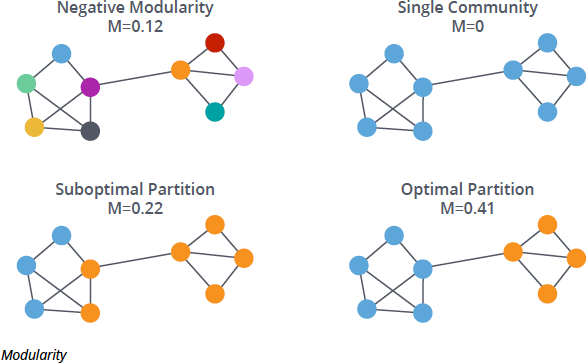
\includegraphics[width=0.5\textwidth]{./img/net/modularity.png}
    \caption{Esempio di modularity.}
    \label{fig:modularity}
\end{figure}
\subsubsection{Hierarchy-centric}
L'obiettivo di questa categoria è quello di costruire una struttura gerarchica
delle community basata sulla topologia della rete.

Questo obiettivo può essere raggiunto utilizzando due approcci differenti:
\begin{itemize}
    \item \textbf{Agglomerative}: si parte da una situazione in cui ogni nodo
          rappresenta una community a sé stante. A questo punto, si uniscono
          le community in base a un criterio di similarità.
    \item \textbf{Divisive}: si parte da una situazione in cui tutti i nodi
          appartengono alla stessa community. A questo punto, si dividono le
          community in base a un criterio di similarità, ad esempio si può usare la centralità come 
          la betweenness.
\end{itemize}
Solitamente, la costruzione di tale struttura, sfrutta la matrice delle distanze,
la quale viene aggiornata, ad ogni iterazione, riducendo la dimensione (eliminando
le colonne e righe dei nodi uniti sotto una community) in modo da creare delle
community.

Il prodotto di questa operazione può essere rappresentato con una struttura ad
albero, detta \textbf{dendrogramma}.
\begin{figure}[!ht]
    \centering
    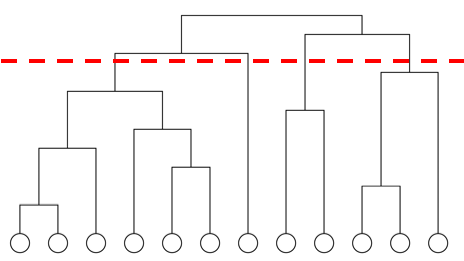
\includegraphics[width=0.5\textwidth]{./img/net/dendrogram.png}
    \caption{Esempio di dendrogramma.}
    \label{fig:dendrogram}
\end{figure}

Un possibile criterio per suddividere la rete è la \textbf{edge-betweeness}, ovvero
il numero di cammini minimi tra ogni coppia di nodi che passa attraverso l'arco
su cui calcolo la metrica.

Un esempio del metodo divisivo è quello Girvan-Newman algorithm sui seguenti passi 
iterativi:
\begin{itemize}
    \item calcola la betweenness per ogni edge del grafo
    \item rimuovi gli edge con betweenness massima (si formano delle community)
    \item si rieseguono i passi precedenti per partizionare ancora le community fino a quando non rimangono 
    solo i singoli nodi.
\end{itemize}
Alla fine si produce la struttura gerarchica del grafo.

\section{Social media Analysis}
Prima di iniziare a presentare gli argomenti di questa sezione riprendiamo
le definizioni di \textbf{hub} e \textbf{spoke}.
\begin{definizione}[\textbf{Hub}]
    Un \textbf{hub} è un nodo con un grado molto alto, ovvero un nodo che è
    connesso a molti altri nodi.
\end{definizione}
\begin{definizione}[\textbf{Spoke}]
    Un \textbf{spoke} è un nodo con un grado molto basso, ovvero un nodo che è
    connesso a pochi altri nodi.
\end{definizione}
Reti che rappresentano domini diversi presentano delle strutture diverse nei
collegamenti tra hub-hub e hub-spoke.

Per iniziare ad analizzare la rete, possiamo stimare la probabilità che un nodo
di un grado $k$ e un nodo di grado $k'$ che siano connessi da un arco. Questo
valore dipende dagli archi della rete.
\begin{equation}
    P(k, k') = \frac{k \cdot k'}{2E}
\end{equation}
dove $E$ è il numero di archi della rete. Questa formula ci permette di dire che
gli hubs sono molto più facilmente collegati tra di loro, rispetto agli spoke.
Quindi se due nodi hanno un grado molto alto, allora è molto probabile che siano
connessi tra di loro.

La rete può essere classificata in base alla tipologia di collegamenti tra i nodi.
Possiamo avere tre tipologie di rete:
\begin{itemize}
    \item \textbf{Assortativa}: avremo una tendenza ad avere hub che si collegano
          tra di loro. Un esempio sono le reti sociali, in cui gli hubs (persone
          famose), tendono a collegarsi tra di loro e gli spoke tendono a collegarsi tra di loro.
    \item \textbf{Neutrale}: rete che ha collegamenti tra due nodi con probabilità
          casuale.
    \item \textbf{Disassortativa}: avremo la tendenza ad avere spoke collegati
          agli hub. Un esempio sono le reti proteiche.
\end{itemize}
Un primo modo di studiare la tipologia della rete è quello di rappresentare
attraverso un grafico i collegamenti tra due nodi rispetto al loro grado. Si
costruisce una matrice in cui nella cella $i, j$ si inserisce il numero di archi
che collegano un nodo di grado $i$ con un nodo di grado $j$.

Questa matrice viene poi normalizzata, dividendo il numero di archi per il numero
totale di archi della rete.

Attraverso la visualizzazione di questa matrice, possiamo capire se la rete è
assortativa, disassortativa o neutrale. Se la matrice presenta sulla diagonale
principale una nuvola di punti allora la rete è assortativa. Al contrario, se
la nuvola è sulla diagonale secondaria, allora la rete è disassortativa. Infine,
se si ha una distribuzione uniforme, allora la rete è neutrale.
\begin{nota}
    Se il grafo è orientato allora non è simmetrica è il contrario.
\end{nota}

Definiamo quindi la matrice $e$ di \textbf{correlazione di grado} ovvero $e_{ij}$
è la probabilità di trovare i nodi di grado $i$ e $j$ agli estremi di un arco scelto 
randomicamente. $e_{ij}$ viene calcolato dividendo il numero di edge che hanno come 
estremità nodi di grado $i$ e $j$ e normalizzando.

In seguito definiremo $q_k$ come la probabilità di trovare un nodo di grado $k$ 
alle estremità di un arco selezionato randomicamente.

$$q_k = \frac{k\cdot p(k)}{\overline{k}}$$

dove:
\begin{itemize}
    \item $k$ è il grado selezionato
    \item $p(k)$ è la probabilità di trovare un nodo con grado $k$
    \item $\overline{k}$ è il grado medio
\end{itemize}

Come sono stati definiti i coefficienti avremo che 
$$\sum_{i=1}^{n}e_{ik} = q_k$$

Possiamo determinare l'assortativa o disassortatività controllando se la seguente
uguaglianza è verificata:
\begin{equation}
    e_{ij} = q_i \cdot q_j
\end{equation}

Quindi la magnitudine della correlazione viene calcolata da:
\begin{equation}
    \sum_{i, k}j\cdot k(e_{ik} - q_i\cdot q_k)
\end{equation}
Il valore ottenuto viene successivamente normalizzata dividendo la formula per:
\begin{equation}
    \sigma^2 = \sum_{k}k^2  - q_k - \left[\sum_{k}kq_k\right]^2
\end{equation}
Si ottiene quindi un valore $r$ compreso tra $-1$ e $1$.
\begin{equation}
    r = \frac{\sum_{i, k}jk(e_{ik} - q_iq_k)}{\sigma^2}
\end{equation}
In base al valore di $r$ possiamo determinare se:
\begin{itemize}
    \item $r > 0$ la rete è assortativa.
    \item $r = 0$ la rete è neutrale.
    \item $r < 0$ la rete è disassortativa.
\end{itemize}
Il motivo per cui si studiano queste proprietà è per capire quanto la rete è
robusta. Ad esempio, vogliamo capire quanto influisce sulla rete se rimuoviamo
un nodo.
\begin{definizione}[\textbf{Giant component}]
    La \textbf{Giant component} è la più grande componente connessa di un grafo.
\end{definizione}
Per studiare la robustezza della rete si procede costruendo una rete in cui si
inseriscono casualmente gli archi della rete di partenza. Quando aggiungiamo un
arco allora i cammini esistenti tra i vari nodi si espandono, aumentando di
conseguenza la Giant component. Se la rete è assortativa, quando aggiungiamo un
arco tra hub allora si avrà un impatto notevole sui cammini della rete perché la
Giant component si paleserà prima nella costruzione. Al contrario, se è
disassortativa allora impiegheremo più tempo per arrivare ad osservare la giant
component.

Quindi si può studiare la comparsa della Giant component in base alle caratteristiche
della rete. Questo permette di studiare le proprietà di costruzione e distruzione
di essa.

Per studiare la resistenza della rete si studia la rimozione dei nodi (\textbf{site
    percolation}) o la rimozione degli archi (\textbf{bond percolation}). In
questo caso studiamo quanto tempo impieghiamo a distruggere la Giant component.
Se elimino un nodo allora cambio il grado della rete. Se l'assortativa si distrugge
più lentamente.